\section{Supplemental Results}
Figure~\ref{fig:inf.default} illustrates incidence rate and cumulative infections
(similar results to Figure~\ref{fig:toroth}),
for two cities identical in: size, $R_0$, and imported/seed cases,
under three vaccination scenarios:
no vaccination, 100\% allocation to city~A, and equal allocation between cities.
Equal allocation minimizes cumulative infections.
\par
Figures~\ref{fig:grid.dci.none}--\ref{fig:grid.rdci.prop} illustrate
cumulative infections averted by day 120 under ``optimal'' vaccine allocation:
versus no vaccination (absolute: \ref{fig:grid.dci.none}, relative: \ref{fig:grid.rdci.none}), and
versus allocation proportional to city size (absolute: \ref{fig:grid.dci.prop}, relative: \ref{fig:grid.rdci.prop}).
\begin{figure}[h]
  \begin{subfigure}{\linewidth}
    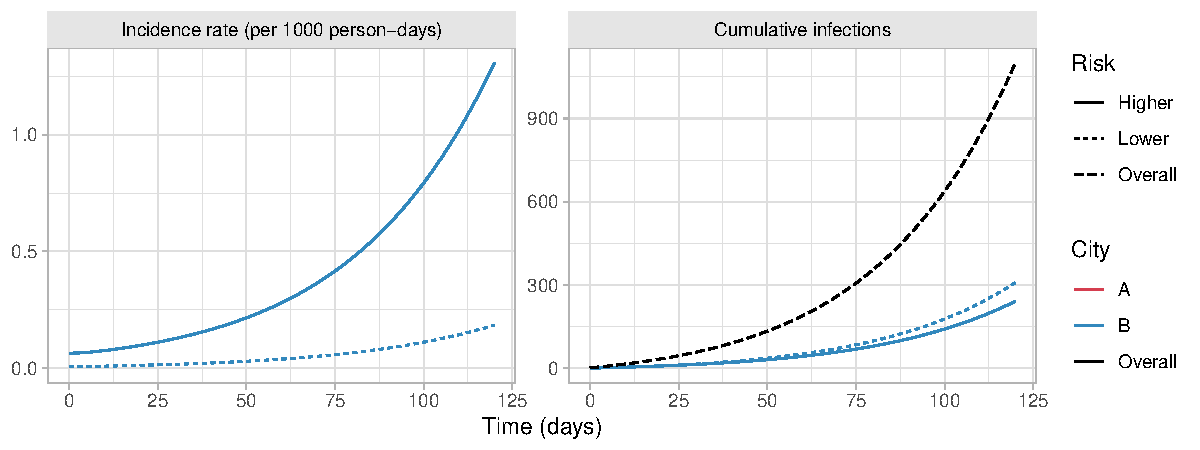
\includegraphics[width=\linewidth]{inf.default.none}
    \caption{No vaccination}
    \label{fig:inf.default.none}
  \end{subfigure}
  \begin{subfigure}{\linewidth}
    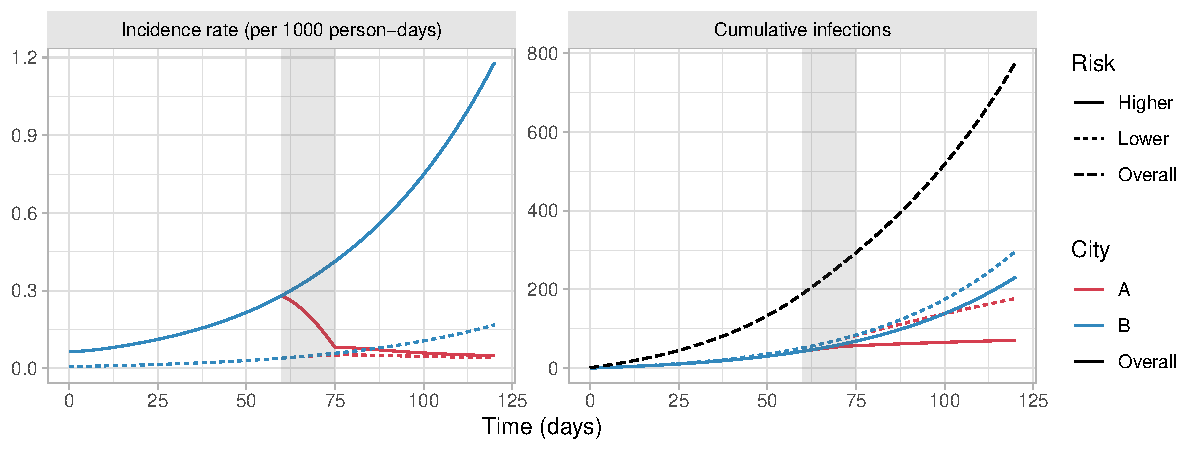
\includegraphics[width=\linewidth]{inf.default.100a}
    \caption{100\% city~A}
    \label{fig:inf.default.100a}
  \end{subfigure}
  \begin{subfigure}{\linewidth}
    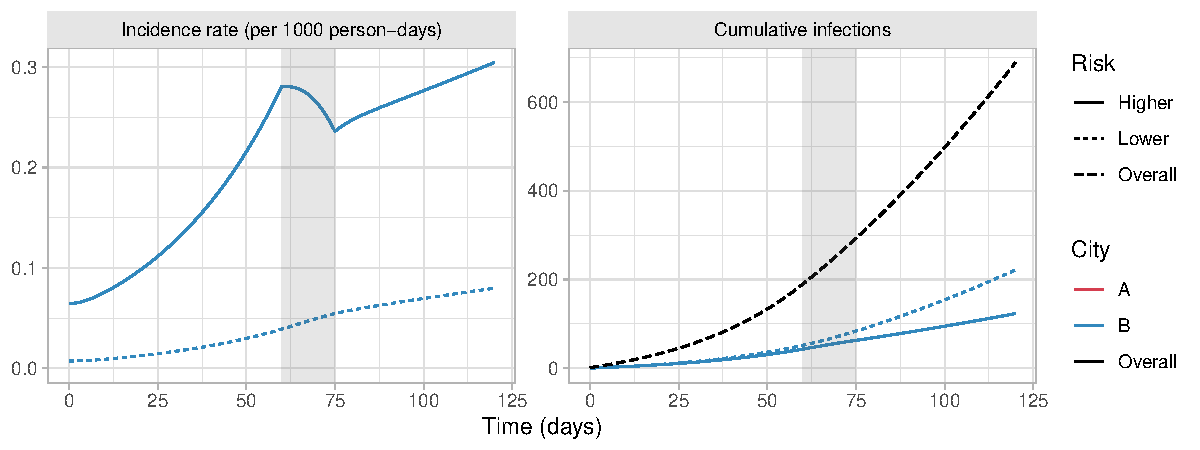
\includegraphics[width=\linewidth]{inf.default.opt}
    \caption{Optimal: 50\% city~A, 50\% city~B}
    \label{fig:inf.default.opt}
  \end{subfigure}
  \caption{Modelled monkeypox incidence and cumulative infections
    in cities A and B with default parameters,
    under two different vaccine allocation scenarios}
  \label{fig:inf.default}
  \floatfoot
  Gray bar indicates period of vaccine roll-out (days 60--75).
\end{figure}
\begin{figure}[h]
  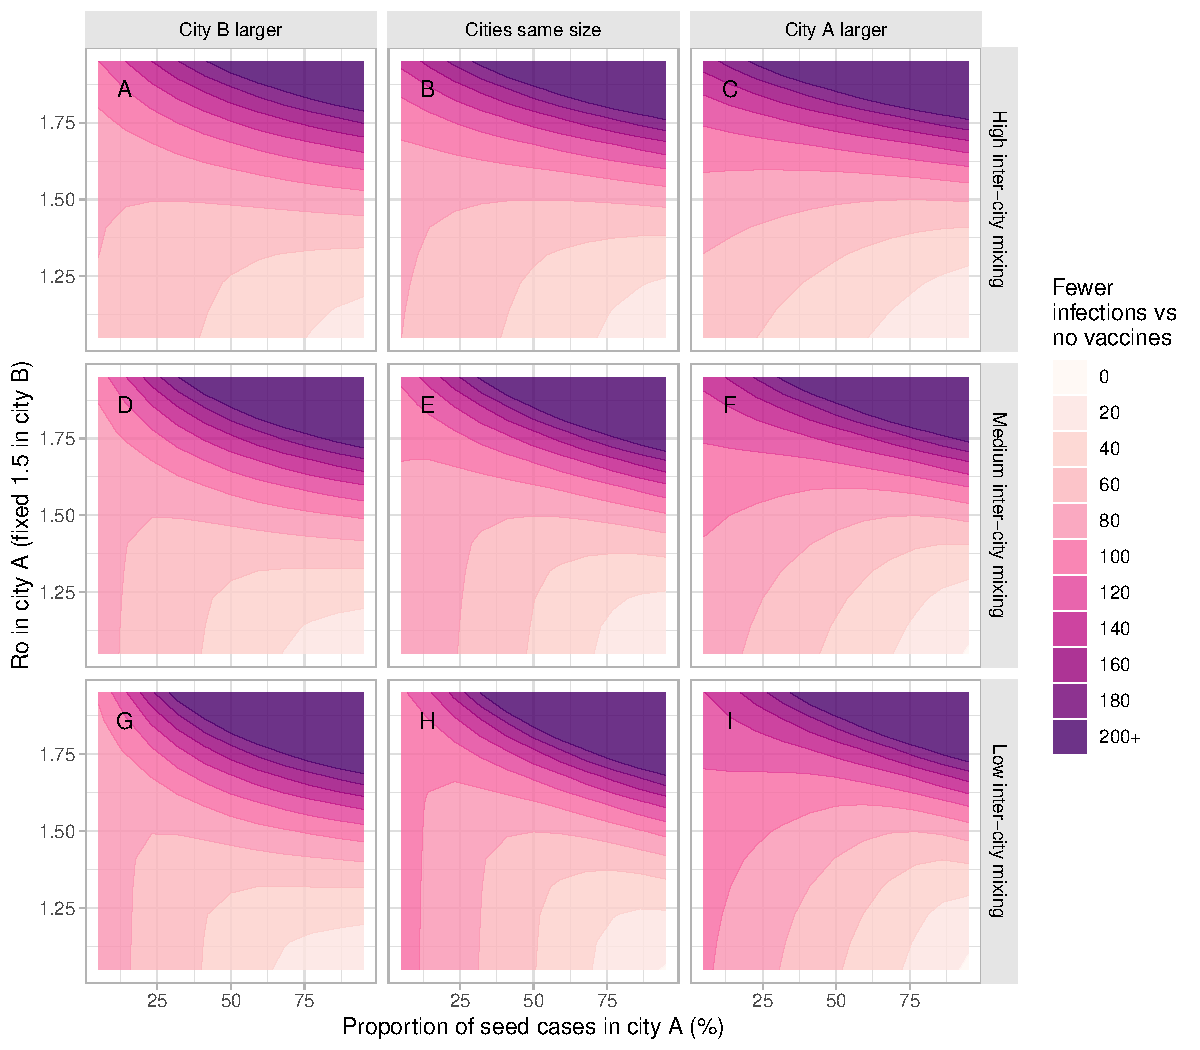
\includegraphics[width=\linewidth]{grid.dci.none.pdf}
  \caption{Absolute fewer infections under optimal vaccine allocation
    versus no vaccination}
  \label{fig:grid.dci.none}
  \floatfoot\gridfoot
\end{figure}
\begin{figure}[h]
  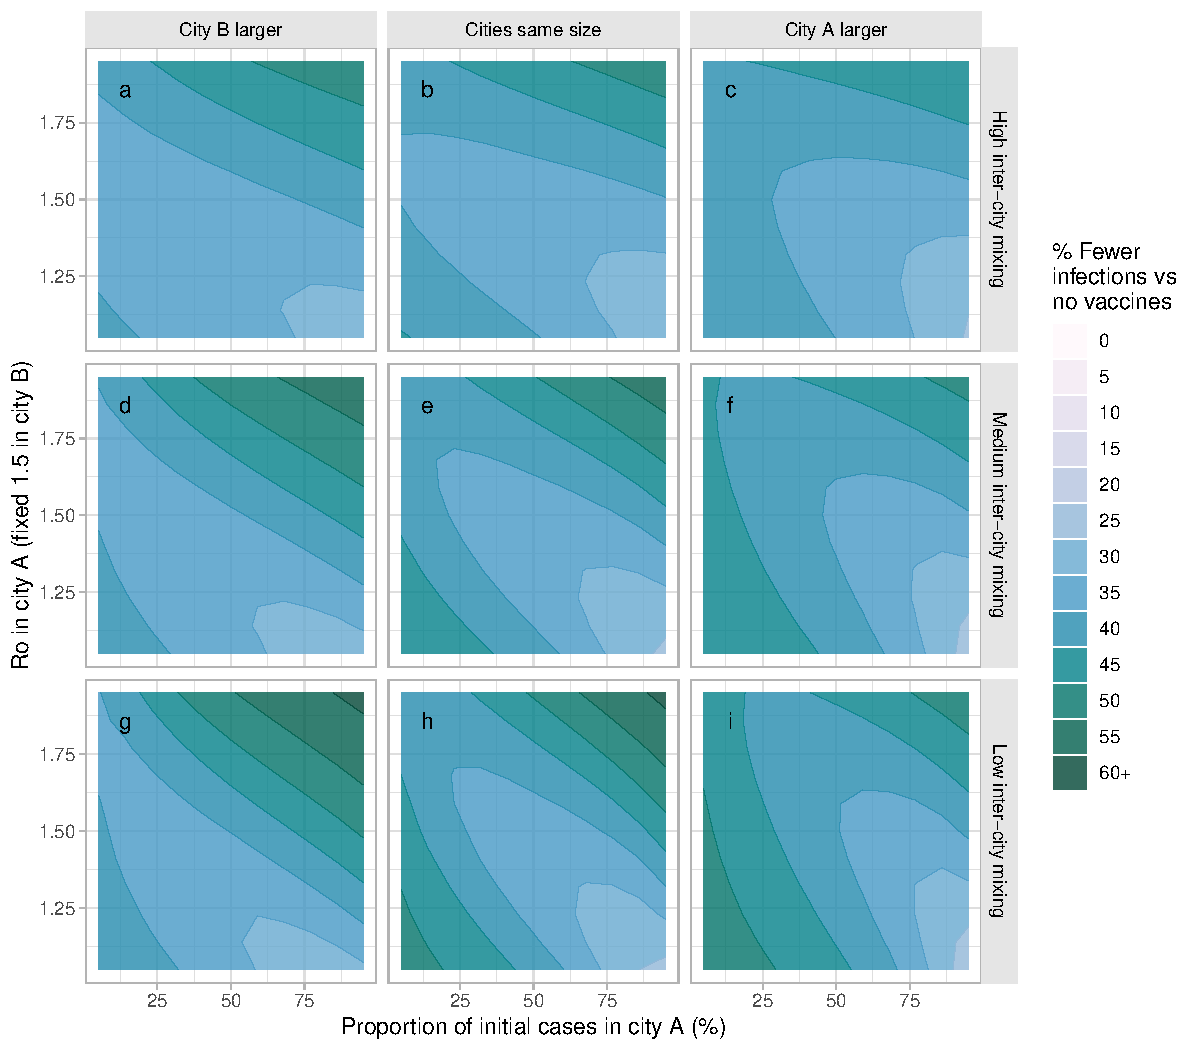
\includegraphics[width=\linewidth]{grid.rdci.none.pdf}
  \caption{Relative fewer infections under optimal vaccine allocation
    versus no vaccination}
  \label{fig:grid.rdci.none}
  \floatfoot\gridfoot
\end{figure}
\begin{figure}[h]
  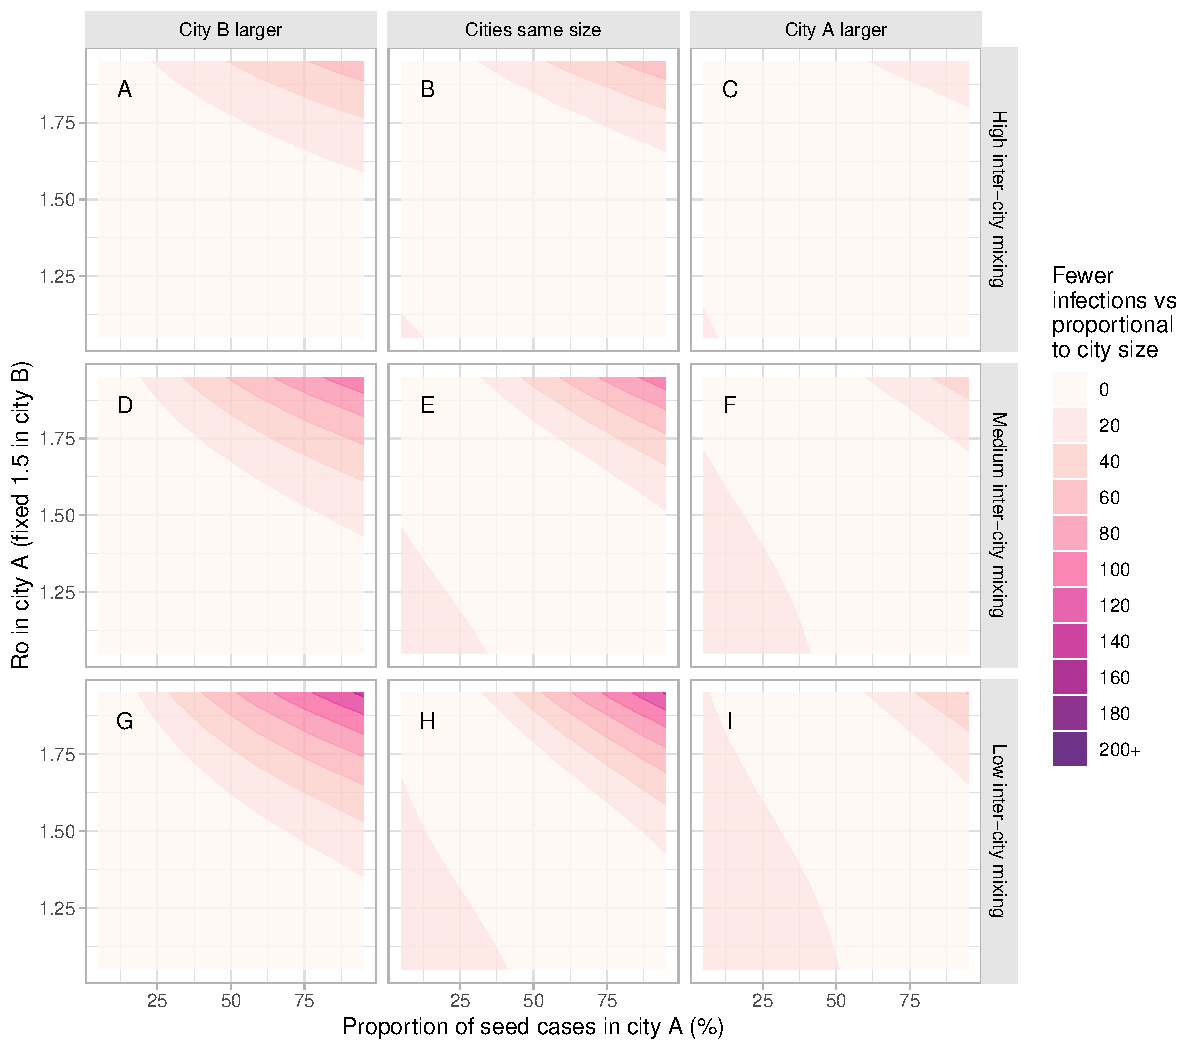
\includegraphics[width=\linewidth]{grid.dci.prop.pdf}
  \caption{Absolute fewer infections under optimal vaccine allocation
    versus allocation proportional to city size}
  \label{fig:grid.dci.prop}
  \floatfoot\gridfoot
\end{figure}
\begin{figure}[h]
  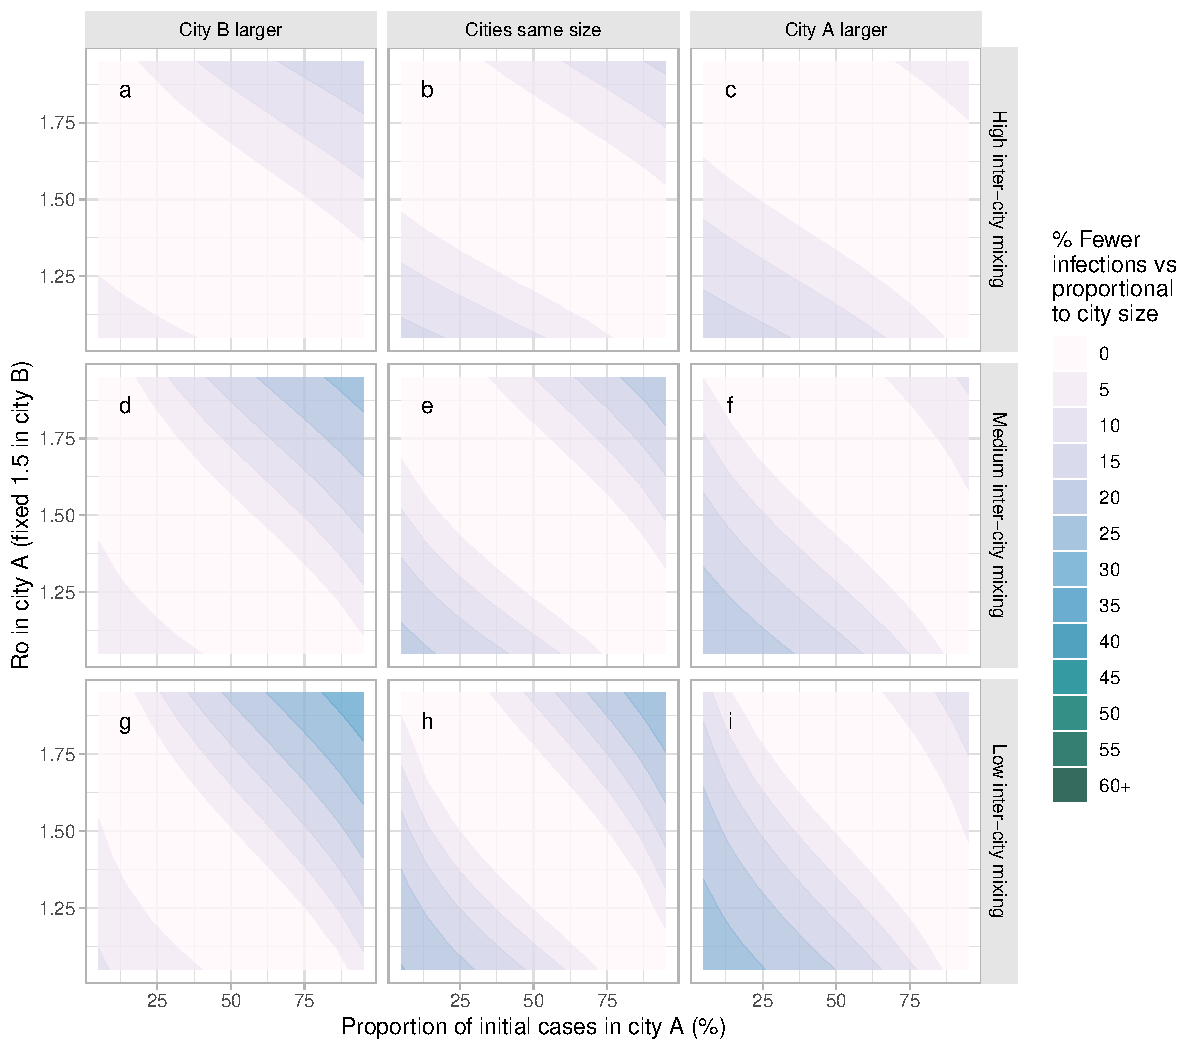
\includegraphics[width=\linewidth]{grid.rdci.prop.pdf}
  \caption{Relative fewer infections under optimal vaccine allocation
    versus allocation proportional to city size}
  \label{fig:grid.rdci.prop}
  \floatfoot\gridfoot
\end{figure}